\documentclass[12pt,dvipdfmx,svgnames,uplatex,aspectratio=169]{beamer}
% \documentclass[12pt,dvipdfmx,svgnames,uplatex,aspectratio=169,handout]{beamer}
%
% ===========================================
% 図・表関係
% ===========================================
% \usepackage[draft]{graphicx}
\usepackage{graphicx}
\graphicspath{{./pics/}}  % \includegraphicsで参照するディレクトリ
%
% ===========================================
% 参考文献
% ===========================================
\usepackage[url=false,isbn=false,doi=false]{biblatex}
% \addbibresource{./bib_textbooks.bib}  % 教科書など
% \addbibresource{./bib_articles.bib}  % 論文など
%
% ===========================================
% 独自スタイルの導入
% ===========================================
\usepackage{/home/ryo/.config/LaTeX/mystyle_beamer}
\newcommand{\git}[1]{{\colorbox{WhiteSmoke}{\texttt{\textbf{#1}}}}}  % gitコマンドを薄い灰色の背景と太字のtypewriterフォントで表記
\newcommand{\stress}[1]{{\colorbox{LightSkyBlue}{#1}}}  % 強調箇所
\setbeamercolor{advanced}{fg=black,bg=Wheat}  % 発展した情報を扱うための色付きbox
%
% ===========================================
% 表紙の記述
% ===========================================
\title{非情報系理系院生のための \\
  モダンな開発環境づくり}
\subtitle{その1. Git/GitHubを使ったソースコード管理}
\author{荒木 亮}
\institute{阪大院基礎工・後藤研}
\date{\today}

% +++++++++++++++++++++++++++++++++++++++++++
% 本文
% +++++++++++++++++++++++++++++++++++++++++++

\begin{document}
\frame{\maketitle}
\begin{frame}{もくじ}
  \tableofcontents
\end{frame}

% ===========================================
% 以下,スライドを記述する
% ===========================================
\section{目標}
\begin{frame}{\insertsection}
  \begin{screen}
    \centering
    ソースコードやLaTeX文書のバージョンを,Git/GitHubで管理する
  \end{screen}

  \begin{itemize}
    \item Gitに初めて触れる人が,「ファイル名に日付をつけてバックアップ」\\「ownCloudに全部おいてる」をGitで代替できるようになることをめざす
  \end{itemize}

  \begin{alertblock}{説明しないこと}
    \begin{itemize}
      \item \git{branch} を使った同時並行的な開発
      \item \git{fork}\(\to\)\git{pull request}\(\to\)\git{merge} を使ったプロジェクト管理
      \item \git{issue},\git{Wiki},\git{Gist}などの便利な機能
    \end{itemize}
    \begin{beamercolorbox}[rounded=true]{advanced}
      \footnotesize{この色の部分は発展的なトピックを扱う}
    \end{beamercolorbox}
  \end{alertblock}
\end{frame}

\section{Gitの構造}
\begin{frame}{\insertsection}
  \centering
  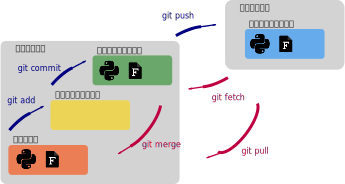
\includegraphics[bb=0.000000 0.000000 979.966736 524.329163, width=120mm]{./pics/git_structure.pdf}
  \begin{flushright}
    \scriptsize{Figures from: \href{https://icon-icons.com/ja/}{icon-icons.com}}
  \end{flushright}
\end{frame}

\begin{frame}{\insertsection}
  \begin{block}{作業ツリー}
    作業をおこなうディレクトリ.
    普通の意味の「フォルダ」
  \end{block}
  \begin{block}{ステージングエリア}
    作業ツリーで編集したファイルの変更点を「とりあえず」保管しておく場所
  \end{block}
  \begin{block}{リポジトリ}
    ファイルを修正履歴も含め保存する場所
  \end{block}
  \begin{block}{ローカルリポジトリ}
    ローカルに保存されているリポジトリ

    ステージングエリアに登録された変更点の集合を「コミット」として保存する
  \end{block}
  \begin{block}{リモートリポジトリ}
    サーバで保存,公開されているリポジトリ

    ユーザのローカルリポジトリと通信し,情報を更新する
  \end{block}
\end{frame}

\section{Gitのコマンド}
\begin{frame}{\insertsection}
  \centering
  \includegraphics[bb=0.000000 0.000000 979.966736 524.329163, width=120mm]{./pics/git_structure_command.pdf}
  \begin{flushright}
    \scriptsize{Figures from: \href{https://icon-icons.com/ja/}{icon-icons.com}}
  \end{flushright}
\end{frame}

\begin{frame}{\insertsection}
  \begin{block}{\git{git add}}
    作業ツリーで編集したファイルの変更点をステージングエリアに追加
  \end{block}
  \begin{block}{\git{git commit}}
    ステージングエリアにある変更点の集合をローカルリポジトリに記録
  \end{block}
  \begin{block}{\git{git push}}
    ローカルリポジトリに記録されたコミット群をリモートリポジトリに送信
  \end{block}
  \begin{block}{\git{git pull}}
    作業ツリーをリモートリポジトリの最新の情報で更新

    \begin{beamercolorbox}[rounded=true]{advanced}
      \footnotesize{
        ローカルリポジトリをリモートリポジトリと同期する\git{fetch}と,

        作業ツリーとローカルリポジトリを統合する\git{merge}コマンドを一つにしたもの
      }
    \end{beamercolorbox}
  \end{block}
\end{frame}

\section{分散型バージョン管理}
\begin{frame}{\insertsection}
  \begin{columns}[c] % 中央をあわせる
    \begin{column}{0.5\textwidth}
      \includegraphics[bb=0.000000 0.000000 600.000000 316.000000, width=60mm]{./pics/multi.png}

      \includegraphics[bb=0.000000 0.000000 589.565143 347.771411, width=60mm]{./pics/intro2_2.png}

      \scriptsize{Figures from: \href{https://owncloud.jp}{ownCloud},\href{https://backlog.com/ja/git-tutorial/}{サルでも分かるGit入門}}
    \end{column}
    \begin{column}{0.5\textwidth}
      \begin{block}{自動更新(クラウドサービス)}
        ローカルの変更箇所を\stress{自動で}\\リモートに送信
      \end{block}
      \hspace{\baselineskip}
      \begin{block}{\git{commit}(Git/GitHub)}
        変更箇所を\stress{任意の段階でまとめ},\\コメントをつけてリモートに送信
        \begin{itemize}
          \item 編集履歴がわかりやすい
          \item 昔の状態の確認や巻き戻しが簡単
          \item 編集が競合したとき,解決が簡単
        \end{itemize}
        \begin{beamercolorbox}[rounded=true]{advanced}
          \footnotesize{
            Gitはファイル情報をリポジトリ内の\texttt{.git/}以下で管理している
            }
        \end{beamercolorbox}
      \end{block}
    \end{column}
  \end{columns}
\end{frame}

\section{なぜGitを使うのか}
\begin{frame}{\insertsection}
  \begin{itemize}
    \item 自動で保存されてしまうクラウドサービスだと…
    \item[] 「前の状態に戻したいけど,いつのを見ればいいんだろう?」
    \item 古い状態を記録しておけないと…
    \item[] 「今は使っていない関数/サブルーチンだけど,また使うかもしれないしとりあえずコメントアウトして残しておこう」
    \item 共同作業で競合がおきてしまうと…
    \item[] 「今からこのファイル編集するから触らないでね!」
    \item[] 「最新のファイルって誰が持ってる?/どこに置いてる?」
  \end{itemize}

  \begin{block}{Gitを使うべきでないファイル}
    \begin{itemize}
      \item 一度作成したらもう編集しないデータ(実験結果,計算データ)
      \item[] \(\to\)(普通の意味での)バックアップで対処
      % \item ソースコード,論文データなど,継続的に改良していくデータ → (Gitなどを使った)バージョン管理
    \end{itemize}
  \end{block}
\end{frame}

\section{今日から始めるGit生活}
\begin{frame}{\insertsection}
  \begin{enumerate}
    \item GitHubでアカウント作成
    \item Github Educationの申請
    \begin{itemize}
      \item[※] 有償アカウントと同等の機能が利用できる
    \end{itemize}
    \item 研究用リポジトリの作成
    \begin{itemize}
      \item[※] Private(非公開)に設定する
      \item[※] プロジェクト単位でリポジトリを作成:全て一つの場所で管理しない
    \end{itemize}
    \item リポジトリをローカルに\git{clone}
    \item フォルダにファイルを追加\(\to\) \git{add} \(\to\) \git{commit} \(\to\) \git{push}
    \begin{itemize}
      \item[※] 見返したときわかりやすいcommitメッセージをつける
    \end{itemize}
    \item GitHubでリモートリポジトリを確認し,コードを確認
  \end{enumerate}
  \begin{beamercolorbox}[rounded=true]{advanced}
    \footnotesize{
      ssh接続やエディタでGit関連の拡張機能を設定しておくと便利
      }
  \end{beamercolorbox}
\end{frame}

\section{便利なGitコマンド}
\begin{frame}{\insertsection}
  \begin{block}{\git{git commit --amend}}
    一旦ローカルリポジトリに登録したコミットを修正
  \end{block}
  \begin{block}{\git{git stash}}
    現在の作業内容を退避し,ステージングエリアの状態を回復

    退避した状態は呼び出せる
  \end{block}
  \begin{block}{\git{git checkout .}}
    作業ツリーの変更点を破棄,ステージングエリアの状態を回復

    ローカルリポジトリに登録された変更点を破棄:\git{git reset --hard}
  \end{block}
  \begin{block}{\git{git reflog}}
    Gitのコマンドログを確認
  \end{block}

  % その他, \git{git revert} \git{git reset}
  % gitコマンドへのオプション,\texttt{.gitignore}
\end{frame}

\section{リンク集}
\begin{frame}{\insertsection}
  \begin{block}{読みやすい順}
    \begin{itemize}
      \item \href{https://backlog.com/ja/git-tutorial/}{サルでもわかるGit入門}
      \item \href{https://www.slideshare.net/matsukaz/git-28304397}{いつやるの?Git入門 v1.1.0}
      \item \href{https://www.slideshare.net/FromAtom/github-26243260}{Github勉強会}
      \item \href{https://git-scm.com/book/ja/v2}{Pro Git book(日本語版)}
      \item \href{https://www.slideshare.net/kotas/git-15276118}{こわくない Git}
    \end{itemize}
  \end{block}
  \begin{block}{For VSCodeユーザー}
    \begin{itemize}
      \item \href{https://qiita.com/jesus_isao/items/63557eba36819faa4ad9}{君には1時間でGitについて知ってもらう(with VSCode)}
      \item \href{https://qiita.com/y-tsutsu/items/2ba96b16b220fb5913be}{VSCodeでのGitの基本操作まとめ}
    \end{itemize}
  \end{block}
  何か疑問・質問があればslackの \texttt{\#50\_github} まで!
\end{frame}

\end{document}
